\documentclass[12pt]{article}

\usepackage[a4paper,margin=1in]{geometry}
\usepackage{amsmath,amssymb}
\usepackage{array}
\usepackage{booktabs}
\usepackage{enumitem}
\usepackage{graphicx}
\usepackage{hyperref}
\usepackage{xcolor}

\hypersetup{
  colorlinks=true,
  linkcolor=black,
  citecolor=blue!50!black,
  urlcolor=blue!50!black
}

\newcolumntype{L}[1]{>{\raggedright\arraybackslash}p{#1}}
\setlength{\emergencystretch}{2em}
\setcounter{tocdepth}{2}

\title{\textbf{Photon-Lensing Morphological Alignment Residual}\\
\large A Synthetic Tau Core Bridge Protocol for Non-Circular Lensing Residual Tests}
\author{Tau Core Research}
\date{Paper 18 draft package, 2026}

\begin{document}
\maketitle

\begin{abstract}
Weak gravitational lensing measures metric and line-of-sight information rather
than ontological matter content directly.  Standard analyses interpret lensing
residuals through mass, nuisance, and systematic models.  Tau Core motivates a
different but claim-safe diagnostic question: if some lensing residual contains
a morphology/readout component, can a source-side morphology template recover
it without being built from the residual itself?

This paper packages a synthetic photon-lensing bridge protocol for a
Morphological Alignment Residual (MAR).  The source-side template is
\[
  T_{\tau}(x)=B_{\rm env}(x)A_f(x)M_{bf}(x),
\]
where \(B_{\rm env}\) is environmental boundary strength, \(A_f\) is filament
strength, and \(M_{bf}=1-(\hat b\cdot\hat f)^2\) is baryon-filament angular
mismatch.  The primary statistic is
\[
  C_{\tau}=Corr(\Delta\kappa,T_{\tau}),
\]
reported against random-orientation, spatial-shuffle, baryon, filament-only,
systematics, and no-Tau controls.

In the included synthetic package, the toy recovery gives
\(C_{\tau}=0.8745\), compared with random-orientation mean \(0.3938\),
spatial-shuffle mean \(0.0123\), baryon-template correlation \(0.0741\), and
filament-only correlation \(0.4015\).  A sensitivity ladder detects injected
\(\epsilon_{\tau}\leq0.01\) in the tested noise ladder.  Realistic stress tests
are weaker: \(Q_{\rm MAR}\) scores are \(5/10\), \(4/10\), \(4/10\), and
\(2/10\) for mild, medium, hard, and no-Tau control cases.  A
systematics-separated ridge regression leaves positive but modest
\(\Delta R^2_{\tau}\) increments for mild/medium/hard cases and a near-zero
increment for the no-Tau control.

These are synthetic protocol statistics.  They are not real-data lensing
detections, dark-matter falsifications, likelihood ratios, or physical
validation of Tau Core.  The contribution is a reproducible non-circular
search grammar for photon-lensing residuals and a concrete bridge from
source-side morphology to future lensing-readout tests.
\end{abstract}

\tableofcontents

\section{Scope and claim boundary}

This manuscript should be evaluated as a synthetic methodology and bridge
protocol paper.  It does not analyze real survey maps, does not detect a
lensing anomaly, does not solve dark matter, and does not prove Tau Core.

\noindent\textbf{Status:} synthetic photon-lensing MAR protocol; not empirical
validation.

The main claim is deliberately narrow:
\begin{quote}
A non-circular source-side morphology template can be defined for lensing
residual tests, and the included synthetic package shows how such a template
survives, weakens, or fails under increasingly strict controls.
\end{quote}

The package is useful because it preserves negative pressure on the hypothesis.
The toy recovery is strong, but the realistic stress and systematics-separated
tests show that systematics, filament-only terms, baryon structure, and
orientation effects can compete with the MAR statistic.  This is a feature of
the paper, not a defect: the protocol is designed to expose where the MAR route
is fragile.

\section{Relation to photon lensing and Tau Core}

In standard lensing, light follows null geodesics of an effective metric, and
observables such as convergence \(\kappa\), shear \(\gamma\), magnification
\(\mu\), deflection \(\alpha\), or time delay are reconstructed from metric and
source geometry \cite{BartelmannSchneider2001,Kilbinger2015,Mandelbaum2018}.
The direct observed object is a lensing observable, not an ontological label
``dark matter'' or ``modified gravity.''

The Tau Core translation used here is only operational:
\[
  \Delta O_{\rm lens}
  =
  {\cal L}_{O}\!\left[\delta g^{\tau}_{\mu\nu}\right],
  \qquad
  O\in\{\alpha,\kappa,\gamma,\mu,\Delta t\}.
\]
Here \(\delta g^{\tau}_{\mu\nu}\) denotes a possible metric/readout residual,
and \({\cal L}_{O}\) denotes the lensing projection operator for observable
\(O\).  This formula is not a derived Tau field equation.  It is a claim-safe
bookkeeping statement: lensing residuals should first be treated as metric or
projection residuals before assigning ontology.

\section{Morphological Alignment Residual}

The MAR hypothesis asks whether a lensing convergence residual
\[
  \Delta\kappa(x)=\kappa_{\rm obs}(x)-\kappa_{\rm base}(x)
\]
contains a component aligned with independently defined morphology handles.
The source-side template is
\[
  T_{\tau}(x)
  =
  B_{\rm env}(x)\,A_f(x)\,M_{bf}(x),
  \label{eq:mar-template}
\]
with
\[
  M_{bf}(x)=1-(\hat b(x)\cdot \hat f(x))^2.
  \label{eq:mismatch}
\]
The square appears because a filament direction is an axis, not an oriented
arrow: \(\hat f\sim-\hat f\).

The important non-circularity rule is:
\[
  T_{\tau}
  =
  F(\hbox{baryon map},\hbox{filament map},\hbox{environment map}),
  \qquad
  T_{\tau}\not=F(\Delta\kappa).
  \label{eq:non-circular}
\]
The recovery statistic is then
\[
  C_{\tau}=Corr(\Delta\kappa,T_{\tau}).
  \label{eq:corr}
\]
This statistic is meaningful only with controls.  A positive \(C_{\tau}\) by
itself is not a Tau Core signal.

\begin{figure}[t]
\centering
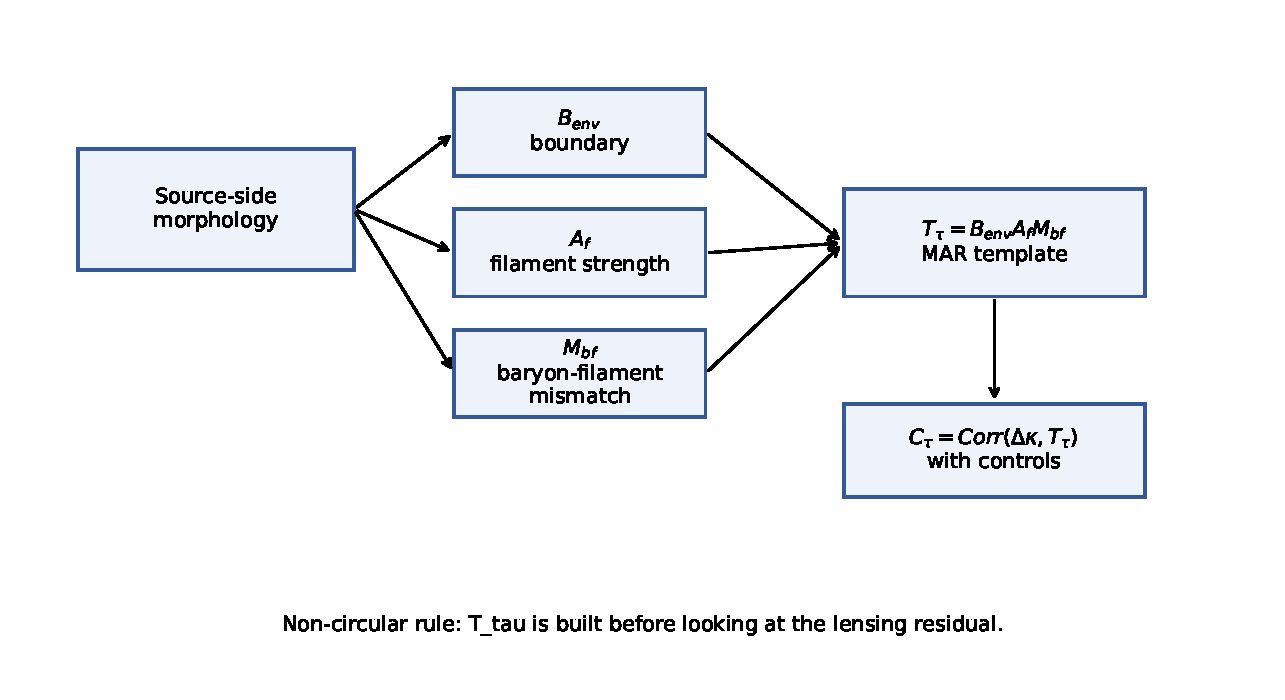
\includegraphics[width=0.95\linewidth]{figures/fig_mar_protocol.pdf}
\caption{MAR protocol.  The source-side template is built from boundary,
filament, and baryon-filament mismatch handles before it is compared with the
lensing residual.  This is the non-circularity condition that distinguishes the
protocol from residual fitting.}
\label{fig:protocol}
\end{figure}

\section{Synthetic generative tests}

The toy generative model is
\[
  \kappa_{\rm obs}
  =
  \kappa_{\rm base}
  +
  \epsilon_{\tau}T_{\tau}
  +
  \eta,
  \label{eq:toy-generator}
\]
so that
\[
  \Delta\kappa
  =
  \kappa_{\rm obs}-\kappa_{\rm base}.
\]
This toy model is intentionally favorable to the MAR statistic: a component
proportional to \(T_{\tau}\) is injected.  Therefore the toy recovery is a
sanity check, not evidence for nature.

\begin{figure}[t]
\centering
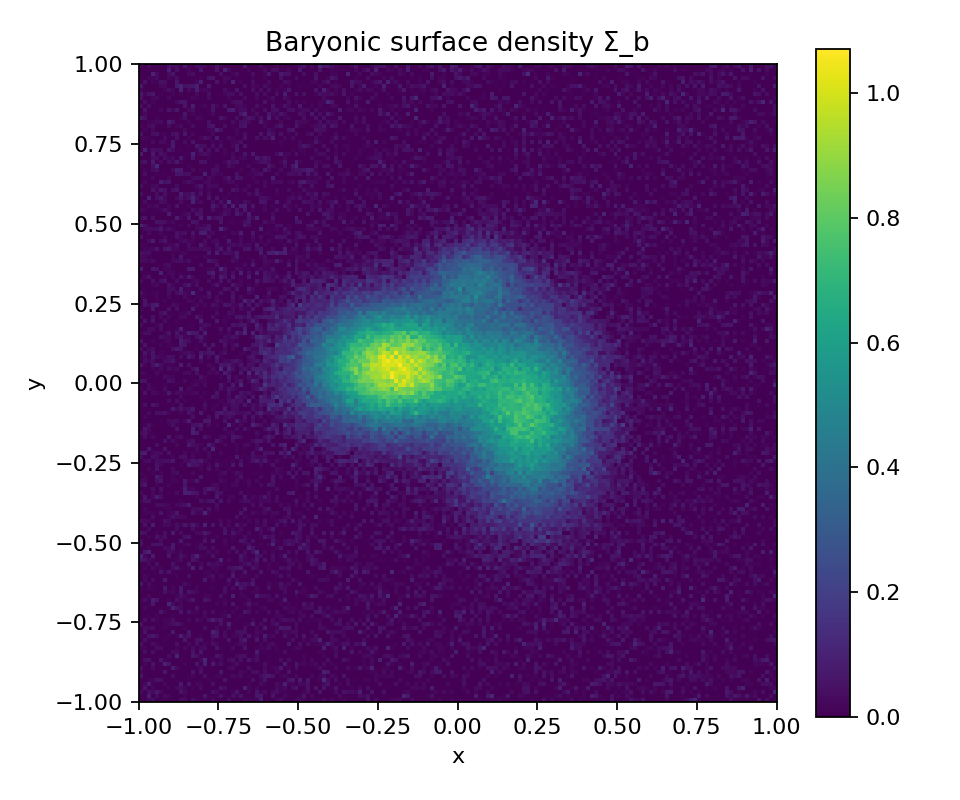
\includegraphics[width=0.48\linewidth]{figures/fig01_baryonic_surface_density.png}
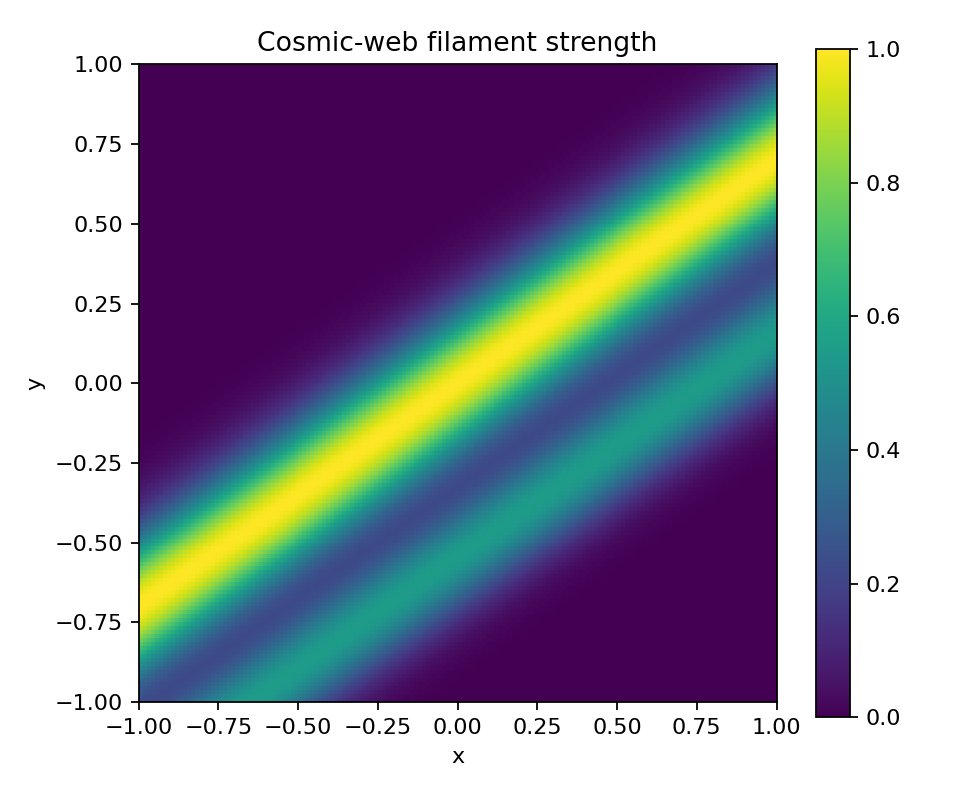
\includegraphics[width=0.48\linewidth]{figures/fig02_filament_strength.png}
\caption{Synthetic source-side inputs from the source package.  Left: baryonic
surface-density-like field.  Right: filament-strength field.  These are
synthetic maps, not survey data.}
\label{fig:inputs}
\end{figure}

\begin{figure}[t]
\centering
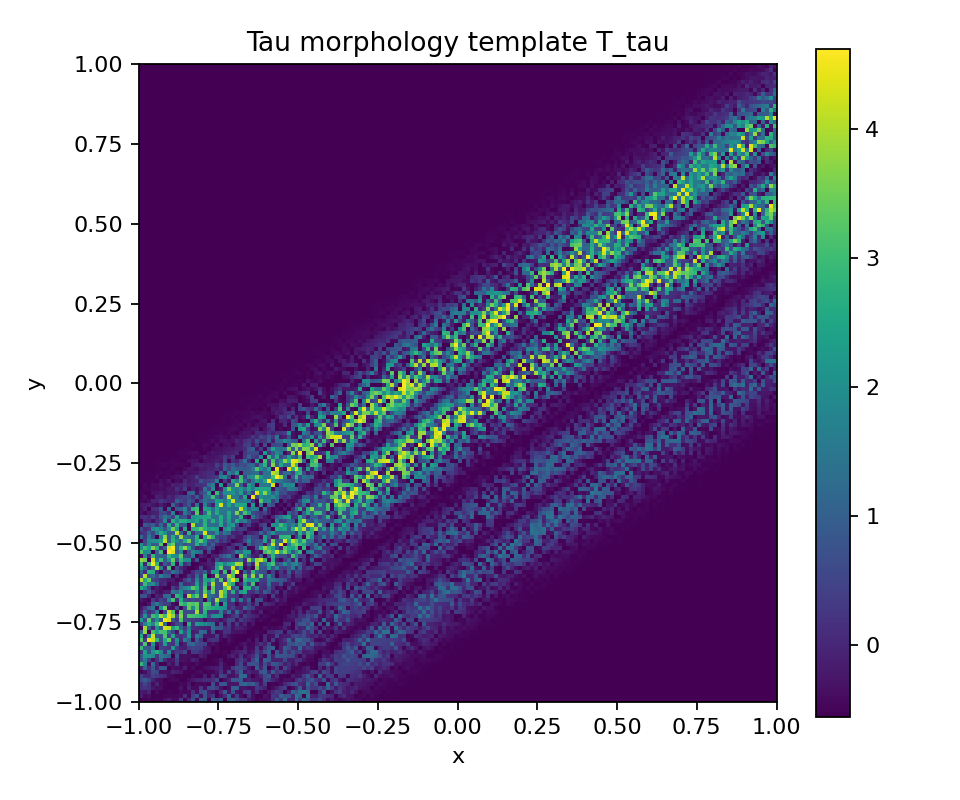
\includegraphics[width=0.48\linewidth]{figures/fig03_tau_template.png}
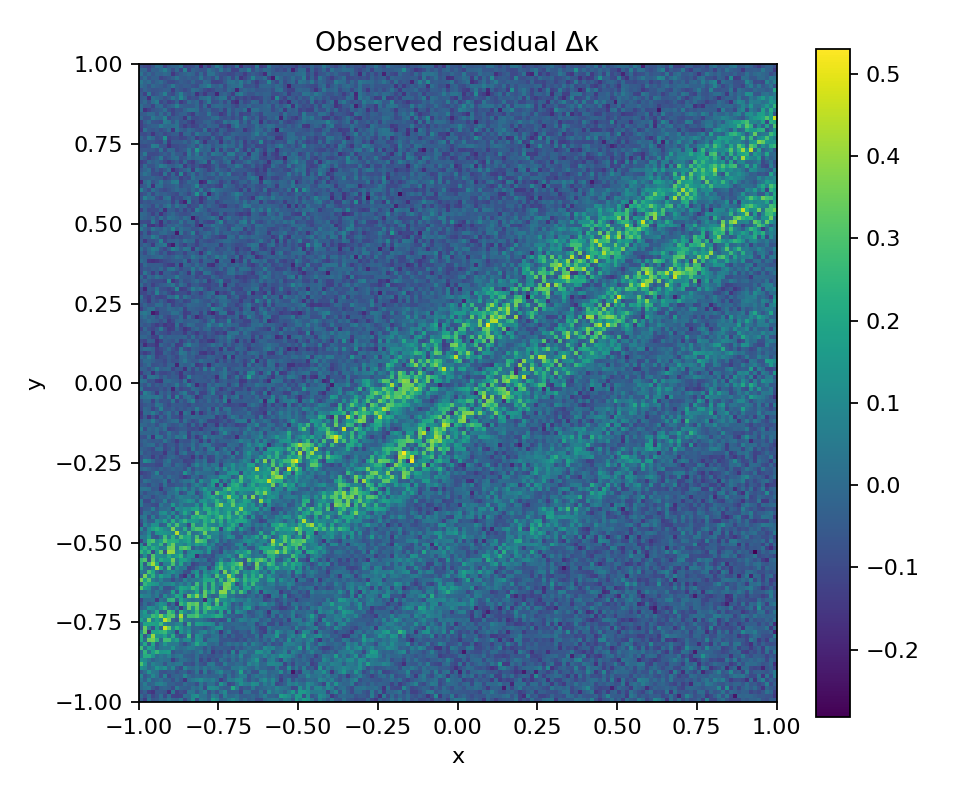
\includegraphics[width=0.48\linewidth]{figures/fig04_lensing_residual.png}
\caption{Synthetic MAR template and synthetic lensing residual.  The residual
contains an injected MAR-like component plus noise.  This figure illustrates
the method, not an observational detection.}
\label{fig:template-residual}
\end{figure}

\subsection{Toy recovery}

The source package reports the toy recovery statistics in
Table~\ref{tab:toy}.  The MAR template recovers the injected component much
more strongly than spatial shuffling or a baryon-only template.  The
filament-only and random-orientation controls are not pure nulls: they retain
part of the morphology structure and therefore remain non-negligible.

\begin{table}[t]
\centering
\small
\begin{tabular}{L{0.45\linewidth}r}
\toprule
Statistic & Value\\
\midrule
\(C_{\tau}=Corr(\Delta\kappa,T_{\tau})\) & 0.8745\\
Random-orientation mean & 0.3938\\
Random-orientation p-value & 0.0010\\
Spatial-shuffle mean & 0.0123\\
Spatial-shuffle p-value & 0.0010\\
Baryon-template correlation & 0.0741\\
Filament-only correlation & 0.4015\\
\bottomrule
\end{tabular}
\caption{Toy MAR recovery.  These are synthetic sanity-check numbers.  They
show that the statistic can recover an injected component, not that a physical
component exists in real data.}
\label{tab:toy}
\end{table}

\section{Sensitivity ladder}

The sensitivity ladder varies the injected amplitude
\[
  \epsilon_{\tau}\in
  \{0,0.005,0.01,0.015,0.02,0.03,0.04,0.06,0.08,0.10,0.12\}
\]
at noise levels \(0.04\), \(0.06\), and \(0.08\).  The package reports minimum
detected amplitudes:
\[
\begin{array}{cc}
\hbox{noise level} & \epsilon_{\tau,\min}\\
\hline
0.04 & 0.010\\
0.06 & 0.010\\
0.08 & 0.005.
\end{array}
\]
The non-monotone threshold ordering is a warning that the ladder is still a
toy audit rather than a calibrated power analysis.

\begin{figure}[t]
\centering
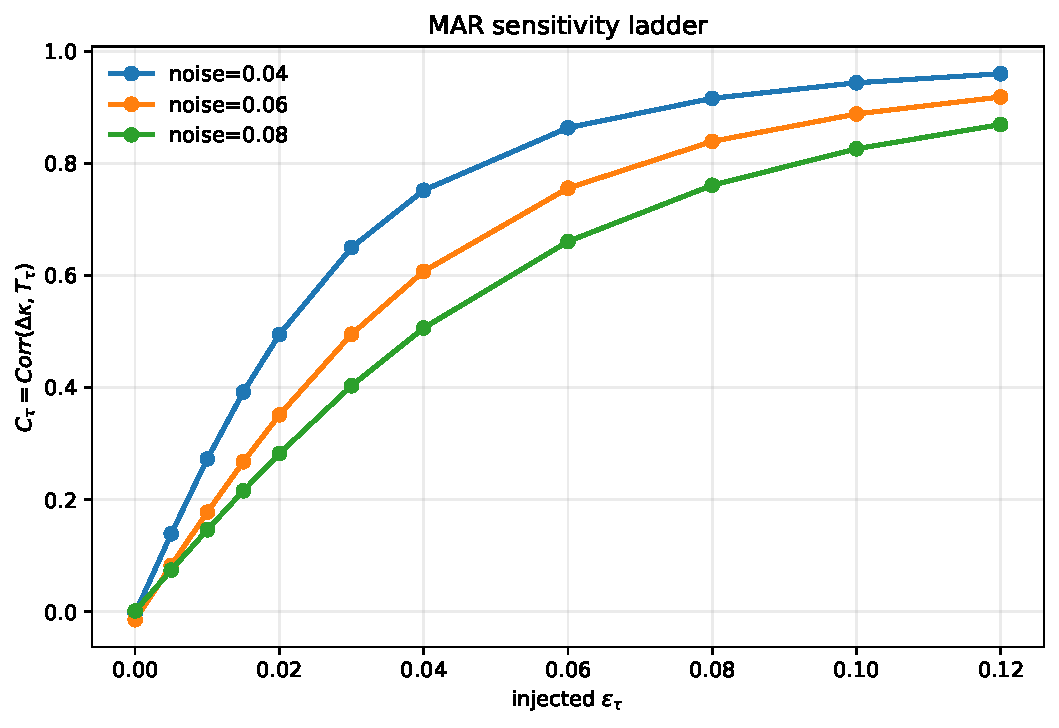
\includegraphics[width=0.86\linewidth]{figures/fig_mar_sensitivity_ladder.pdf}
\caption{Recomputed sensitivity ladder from the compact CSV artifacts.  The
correlation \(C_{\tau}\) increases with injected MAR amplitude in the toy
generator.}
\label{fig:sensitivity}
\end{figure}

\section{Realistic stress test}

The stress test adds correlated noise, a PSF/systematics-like contaminant,
noisy baryonic input, filament orientation errors, imperfect halo/baseline
modeling, smoothing, and a no-Tau control.  The measured residual is no longer
the clean toy residual:
\[
  \Delta\kappa_{\rm meas}
  =
  \kappa_{\rm obs}
  -
  \kappa_{\rm base,model}.
\]
The measured template is also imperfect:
\[
  T_{\tau,{\rm meas}}\neq T_{\tau,{\rm true}}.
\]

The stress-test summary is shown in Table~\ref{tab:stress}.  MAR support
survives mildly, but the score is modest and the systematic template is
competitive or dominant in some cases.  The no-Tau control has lower MAR score
and negative \(C_{\rm real}\), which is the desired sanity check.

\begin{table}[t]
\centering
\small
\begin{tabular}{L{0.22\linewidth}rrrrr}
\toprule
Scenario & \(C_{\rm real}\) & \(p_{\rm shuffle}\) & \(p_{\rm orient}\) &
\(C_{\rm sys}\) & \(Q_{\rm MAR}\)\\
\midrule
mild & 0.3098 & 0.0033 & 0.0033 & 0.2320 & 5\\
medium & 0.2684 & 0.0033 & 0.0033 & 0.3045 & 4\\
hard & 0.1494 & 0.0033 & 0.0033 & 0.3840 & 4\\
no-Tau control & -0.0226 & 0.6279 & 0.0598 & 0.2695 & 2\\
\bottomrule
\end{tabular}
\caption{Realistic stress-test summary.  \(Q_{\rm MAR}\) is a package-local
0--10 stress score, not a universal statistic.  The hard case illustrates the
main vulnerability: systematics can dominate the MAR-like correlation.}
\label{tab:stress}
\end{table}

\begin{figure}[t]
\centering
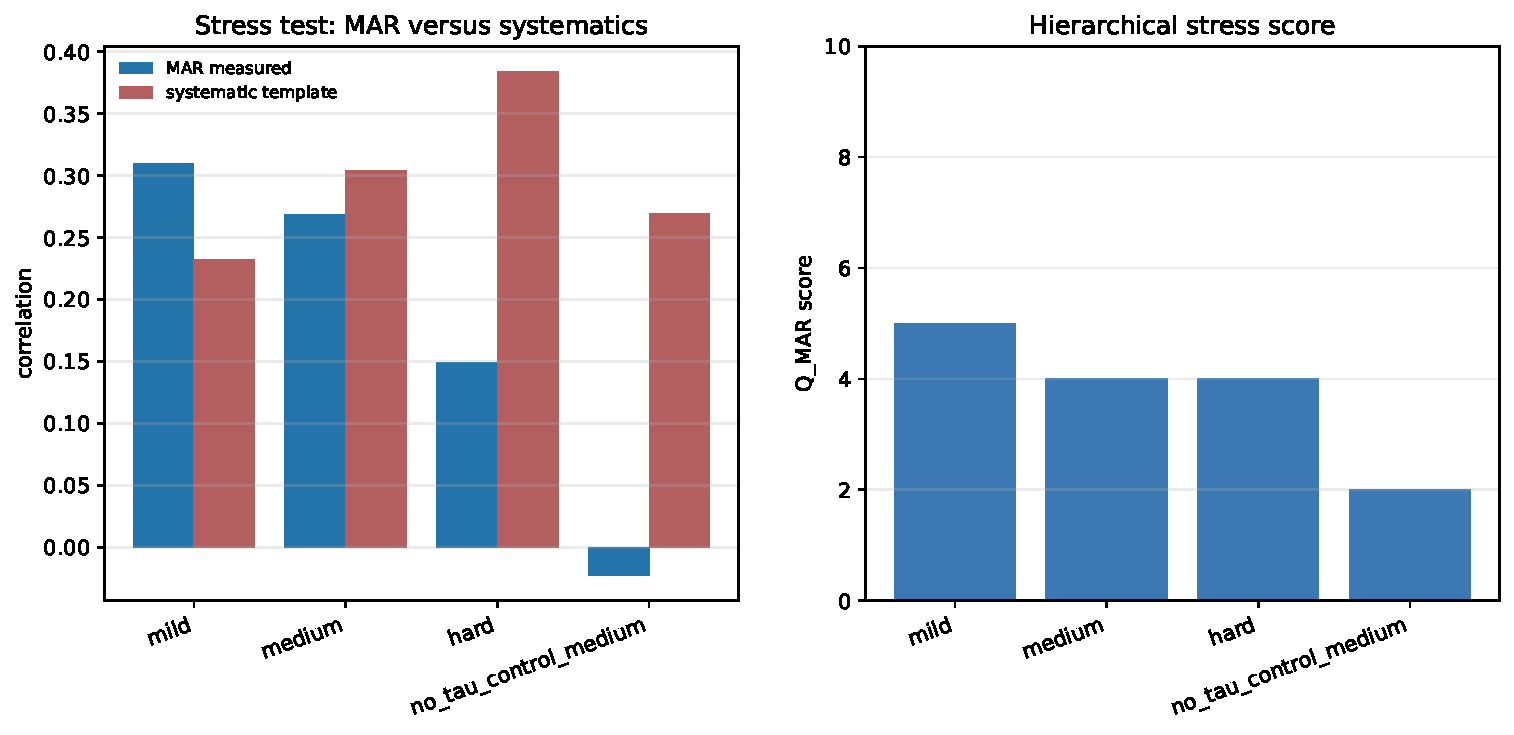
\includegraphics[width=0.95\linewidth]{figures/fig_mar_stress_summary.pdf}
\caption{Stress-test summary.  Left: measured MAR correlation compared with
systematics-template correlation.  Right: package-local hierarchical
\(Q_{\rm MAR}\) score.}
\label{fig:stress}
\end{figure}

\section{Systematics-separated regression}

A stronger check asks whether the Tau template contributes after standard
control templates are included.  The package uses a ridge-style regression
grammar:
\[
  \Delta\kappa
  =
  a_{\tau}T_{\tau}
  +
  a_{\rm sys}S
  +
  a_bB
  +
  a_fF
  +
  a_{\rm bd}D
  +
  \epsilon.
\]
The relevant statistic is the incremental explanatory power:
\[
  \Delta R^2_{\tau}
  =
  R^2_{\rm full\ with\ tau}
  -
  R^2_{\rm no\ tau\ controls}.
\]

\begin{table}[t]
\centering
\small
\begin{tabular}{L{0.25\linewidth}rrrr}
\toprule
Scenario & \(\Delta R^2_{\tau}\) & \(p_{\rm perm}\) &
partial corr. & \(a_{\tau}\)\\
\midrule
mild & 0.0537 & 0.0083 & 0.2821 & 0.2925\\
medium & 0.0220 & 0.0083 & 0.1832 & 0.1841\\
hard & 0.0097 & 0.0083 & 0.1130 & 0.1235\\
no-Tau control & 0.000001 & 0.9669 & -0.0008 & -0.0009\\
\bottomrule
\end{tabular}
\caption{Systematics-separated regression.  The Tau-template increment remains
positive in the injected scenarios and collapses in the no-Tau control, but the
increment becomes small in the hard case.}
\label{tab:systematics}
\end{table}

\begin{figure}[t]
\centering
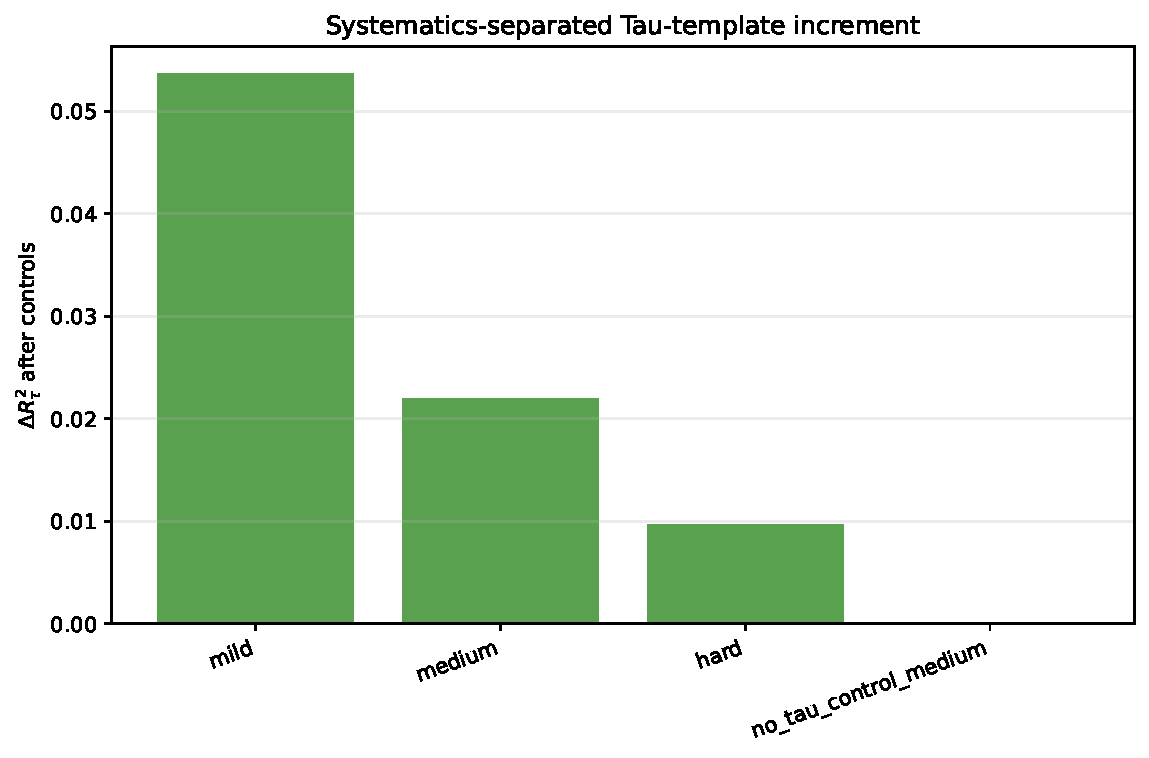
\includegraphics[width=0.82\linewidth]{figures/fig_mar_delta_r2_after_controls.pdf}
\caption{Incremental \(R^2\) supplied by the Tau template after control
templates are included.  The no-Tau control is near zero.}
\label{fig:delta-r2}
\end{figure}

\section{Connection to Paper 17}

Paper 17 separated shared-parent covariance \(Z_{\rm shared}\) from
morphology/orientation support \(Z_{\rm orient}\).  Paper 18 should be read in
that discipline.  MAR is not evidence simply because a filamentary template
correlates with a residual.  In a future real-data endpoint, MAR would need to
be reported in a two-axis form:
\[
  (Z_{\rm shared}^{\rm MAR}, Z_{\rm orient}^{\rm MAR}).
\]
Only the shared-parent or residual-covariance axis can promote the candidate.
The morphology/orientation axis can only reinforce or diagnose it.

\section{Required real-data upgrade}

The package is not ready for real-data claims.  A serious upgrade would need:
\begin{enumerate}[leftmargin=1.4em]
\item source-native weak-lensing or CMB-lensing maps
\cite{KiDS1000,DESY3,ACTDR6Lensing};
\item source-native galaxy/filament/environment maps, masks, and redshift bins
\cite{DESI2016};
\item survey covariance, shape noise, photo-\(z\), PSF/foreground and selection
systematics;
\item blind construction of \(T_{\tau}\) before scoring \(\Delta\kappa\);
\item no-Tau, baryon-only, filament-only, random-orientation, mask-only, and
systematics-template controls;
\item mock injection with known MAR and non-MAR components;
\item held-out scoring and independent implementation.
\end{enumerate}
Until those conditions are met, the status remains:
\[
  \texttt{SYNTHETIC\_PHOTON\_LENSING\_MAR\_PROTOCOL\_ONLY}.
\]

\section{Reproducibility package}

The repository provides a one-command reproduction path:
\[
  \texttt{python scripts/reproduce.py}.
\]
The command rebuilds the summary artifacts, regenerates figures, compiles the
PDF, builds the arXiv source zip, and runs public smoke tests.

The original package section and figures are preserved under
\[
  \texttt{source\_package\_docs/},\qquad
  \texttt{source\_package\_figures/}.
\]
The paper uses only compact derived CSV artifacts under
\[
  \texttt{data/derived/}.
\]

\section{Conclusion}

Paper 18 records a synthetic photon-lensing MAR bridge protocol.  The protocol
is stronger than a note because it supplies a concrete non-circular template,
a toy recovery, a sensitivity ladder, a realistic stress test, a
systematics-separated regression, and explicit failure conditions.

The claim remains narrow.  The paper does not prove Tau Core and does not
detect a lensing residual in real data.  Its contribution is methodological:
it defines how a Tau Core-inspired photon-lensing morphology residual could be
searched for without fitting the residual into the template, and it shows that
the route is promising in toy data but vulnerable to realistic systematics.
The next scientific step is a source-native mock-catalog and survey-mask
implementation with the MAR template frozen before endpoint scoring.

\bibliographystyle{plain}
\bibliography{refs}

\end{document}
